\documentclass{article}


\usepackage{PRIMEarxiv}
\usepackage{todonotes}
\usepackage[utf8]{inputenc} % allow utf-8 input
\usepackage[T1]{fontenc}    % use 8-bit T1 fonts
\usepackage{hyperref}       % hyperlinks
\usepackage{url}            % simple URL typesetting
\usepackage{booktabs}       % professional-quality tables
\usepackage{amsfonts}       % blackboard math symbols
\usepackage{nicefrac}       % compact symbols for 1/2, etc.
\usepackage{microtype}      % microtypography
\usepackage{lipsum}
\usepackage{subfiles}
\usepackage{fancyhdr}       % header
\usepackage{graphicx}       % graphics
\usepackage{algpseudocodex}
\usepackage{algorithm}
\usepackage{amsmath, amssymb}
\graphicspath{{media/}}     % organize your images and other figures under media/ folder

%Header
\pagestyle{fancy}
\thispagestyle{empty}
\rhead{ \textit{ }} 

% Update your Headers here
\fancyhead[LO]{Neural Search Indexing Optimization: Integrating Augmentation and PEFT for Efficient Retrieval}
% \fancyhead[RE]{Firstauthor and Secondauthor} % Firstauthor et al. if more than 2 - must use \documentclass[twoside]{article}

  
%% Title
\title{Neural Search Indexing Optimization: Integrating Augmentation and PEFT for Efficient Retrieval}

\author{
  Alessio Borgi, Eugenio Bugli, Damiano Imola \\
  1952442, 1934824, 2109063 \\
  Sapienza Università di Roma \\
  \texttt{\{borgi.1952442, bugli.1934824, imola.2109063\}@studenti.uniroma1.it} \\
}

\begin{document}
\maketitle

\begin{abstract}


This project presents a novel approach to enhancing the Differentiable Search Index (DSI), a neural inverted index framework, by introducing three data augmentation techniques: (1) converting numerical values to words (Num2Word), (2) removing stopwords, and (3) leveraging a Part of Speech Masked Language Modeling (POS-MLM) strategy. These augmentations aim to improve the robustness and effectiveness of the DSI model in diverse retrieval scenarios. Additionally, we propose and evaluate four advanced variants of the DSI model: DSI+LoRA, DSI+QLoRA, DSI+AdaLoRA, and DSI+ConvoLoRA, which integrate parameter-efficient fine-tuning methods to optimize performance and resource utilization.


\end{abstract}

% keywords can be removed
\keywords{DSI \and POS-MLM \and Dynamic Pruning \and LoRA \and QLoRA \and AdaLoRA \and ConvoLoRA}

\section{Introduction} \subfile{sections/intro.tex}
\section{Dataset} \subfile{sections/data.tex}
\begin{figure*}
  \centering
  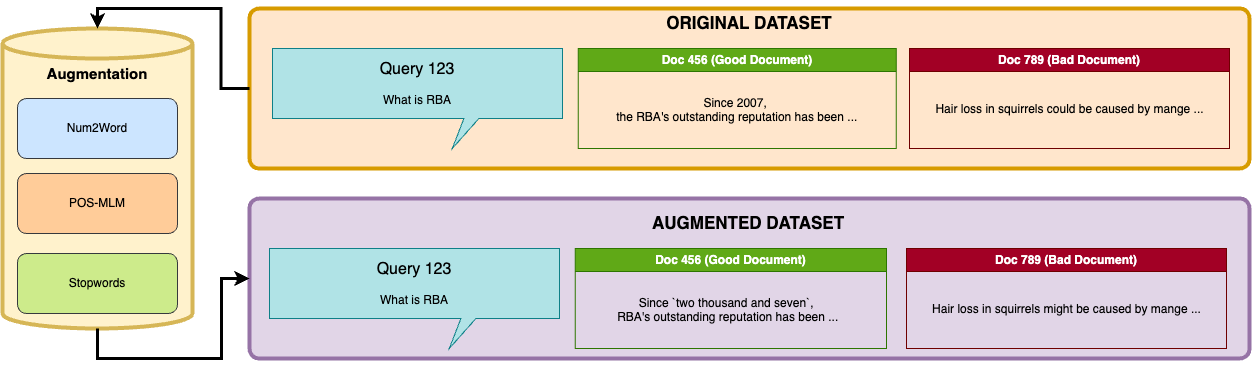
\includegraphics[width=\textwidth]{figs/dataset.png}
  \caption{Data Augmentation Pipeline.}
  \label{fig:fig1}
\end{figure*}
\section{Model} \subfile{sections/model.tex}
\section{Training and Results} \subfile{sections/training.tex}



\section{Conclusion}
In this work, we enhanced the Differentiable Search Index (DSI) by integrating novel data augmentation techniques and parameter-efficient fine-tuning (PEFT) methods to improve retrieval effectiveness and computational efficiency. Our augmentation strategies, including Num2Word transformation, stopword removal, and POS-MLM augmentation, enriched semantic representations, reducing noise and improving contextual understanding. 

In parallel, we leveraged PEFT techniques such as LoRA, QLoRA, AdaLoRA, and ConvLoRA to optimize training and inference, reducing memory consumption while preserving retrieval accuracy. 

Future research will focus on extending these optimizations to larger datasets, refining augmentation techniques, and exploring further parameter-efficient methodologies to enhance retrieval capabilities in real-world applications.




%Bibliography
\bibliographystyle{unsrt}  
\bibliography{references}  


\end{document}
